\subsection{Nekřížení hladin --- dvouhladinový systém}\index{teorém!nekřížení hladin}
\label{sec:AvoidedCrossing}
Hamiltonián popisující dvouhladinový systém je zadán reálnou maticí
\begin{equation}
    \matrix{H}_{0}
        =\makematrix{e & 0 \\ 0 & -e}
        =e\matrix{\sigma}_{3},
\end{equation}
jejíž vlastní čísla jsou $\pm e\in\mathbb{R}$ a odpovídající normalizované vlastní vektory
\begin{equation}
    \ket{e_{+}}
        =\makematrix{1 \\ 0},\qquad
    \ket{e_{-}}
        =\makematrix{0 \\ 1}.
\end{equation}
K matici $\matrix{H}_{0}$ je přidána interakce ve tvaru
\begin{equation}
    \matrix{H}_{\ti{I}}
        =\makematrix{0 & v \\ v & 0}
        =v\matrix{\sigma}_{1},
\end{equation}
kde $v,w\in\mathbb{R}$.

\begin{enumerate}
\item 
    Spočítejte vlastní hodnoty $E_{+},E_{-}$ ($E_{-}\leq E_{+}$) a odpovídající \emph{normalizované} vlastní vektory $\ket{E_{+}}, \ket{E_{-}}$ systému popsaného maticí $\matrix{H}=\matrix{H}_{0}+\matrix{H}_{\ti{I}}$.

\item 
    Zakreslete závislost energetických hladin $E_{\pm}$ na parametru $v$ a určete vlastní vektory $\ket{E_{\pm}(v)}$ 
    pro (a) $v=0$, (b) $v\rightarrow\pm\infty$.

\item 
    Zakreslete závislost energetických hladin $E_{\pm}$ na parametru $e$ a určete vlastní vektory $\ket{E_{\pm}(e)}$ pro (a) $e=0$, 
    (b) $e\rightarrow\pm\infty$.
    Uvažujte dva podpřípady: (a) $v=0$ (křížení hladin) a (b) $v\neq0$ (hladiny se nekříží).    
\end{enumerate}

\begin{note}
    Vzhledem ke tvaru Hamiltoniánu by závislosti $\ket{E_{\pm}(\nu)}$ a $\ket{E_{\pm}(e)}$ měly být hladké funkce.
\end{note}

\begin{solution}
	\begin{enumerate}
	\item
		Spektrum matice $\matrix{H}$ se spočítá z charakteristické rovnice
		\begin{equation}
			\det\makematrix{e-E & v \\ v & -e-E}
				=(E-e)(E+e)-v^{2}
				=0,
		\end{equation}
		jejíž řešení jsou
		\begin{equation}
            E_{\pm}=\pm\sqrt{e^{2}+v^{2}}.
		\end{equation}
        Odpovídající normalizované vlastní vektory lze vyjádřit ve tvaru
        \begin{subequations}
            \begin{align}
                \ket{E_{-}}
                    &=\alpha\makematrix{1 \\ 0}+\beta\makematrix{0 \\ 1}
                    =\makematrix{\alpha \\ \beta},\\
                \ket{E_{+}}
                    &=\beta\makematrix{1 \\ 0}-\alpha\makematrix{0 \\ 1}
                    =\makematrix{\beta \\ -\alpha},\\
                \abs{\alpha}^{2}+\abs{\beta}^{2}
                    &=1,
            \end{align}
        \end{subequations}
        kde
        \begin{subequations}
            \begin{align}
                \alpha
                    &=\frac{\xi}{\sqrt{\xi^2+\left(1+\sqrt{\xi^{2}+1}\right)^{2}}}, &
                \beta
                    &=\frac{1+\sqrt{\xi^{2}+1}}{\sqrt{\xi^2+\left(1+\sqrt{\xi^{2}+1}\right)^{2}}}, &			
                \xi
                    &=\frac{v}{e},
                \label{eq:TwoLevelXi}\\
                \alpha
                    &=\frac{1}{\sqrt{1+\left(\eta+\sqrt{1+\eta^{2}}\right)^{2}}}, &
                \beta
                    &=\frac{\eta+\sqrt{1+\eta^{2}}}{\sqrt{1+\left(\eta+\sqrt{1+\eta^{2}}\right)^{2}}}, &
                \eta
                    &=\frac{e}{v}
            \label{eq:TwoLevelEta}
            \end{align}
            \label{eq:TwoLevelEV}
        \end{subequations}
		($\xi$ a $\eta$ jsou bezrozměrné parametry definované na základě zadaných parametrů $\nu$ a $e$).\sfootnote{
            Vlastní vektory lze také vyjádřit ve tvaru
            \begin{equation}
                \ket{E_{-}}=\makematrix{\cos\phi \\ \sin\phi},\quad
                \ket{E_{+}}=\makematrix{\sin\phi \\ -\cos\phi},
            \end{equation}
            kde
            \begin{equation}
                \phi=\frac{1}{2}\arctan\frac{v}{e}.
            \end{equation}
        }
		
	\item 
		Funkční závislost energetických hladin $E_{\pm}$ je zcela identická jak pro parametr $e$ ($\eta$), tak pro parametr $\nu$ ($\xi$).
        Limitní hodnoty komponent vlastních vektorů jsou podle vztahu~\eqref{eq:TwoLevelEta}
        \begin{subequations}
            \begin{align}
                \alpha(\xi\rightarrow\pm\infty)
                    &=\pm\frac{1}{\sqrt{2}} & \alpha(\xi=0)&=0, \\
                \beta(\xi\rightarrow\pm\infty)
                    &=+\frac{1}{\sqrt{2}} & \beta(\xi=0)&=1
            \end{align}
        \end{subequations}
		a jsou znázorněny na obrázku~\ref{fig:TwoLevelAB}(a).
		Dynamika hladin a limitní tvar vlastních vektorů jsou znázorněny na obrázku~\ref{fig:TwoLevelLD}(a).
		Vlastní vektory $\ket{E_{-}}$ a $\ket{E_{+}}$ se prohodí při přechodu $\xi$ od $-\infty$ k $+\infty$, 
		zatímco energetické hladiny se nepřekříží.
		Jeden z vektorů navíc získá dodatečnou fázi $-1$.\index{teorém!o nekřížení hladin}
		
	\item 
        Pro proměnnou vzdálenost počátečních hladin $e$ a konstantní $\nu$ platí podle vztahu~\eqref{eq:TwoLevelXi} za předpokladu $v\neq0$
        \begin{subequations}
            \begin{align}
                \alpha(\eta\rightarrow-\infty)
                    &=\beta(\eta\rightarrow+\infty)=1, \\
                \alpha(\eta\rightarrow+\infty)
                    &=\beta(\eta\rightarrow-\infty)=-1, \\
                \alpha(\eta=0)
                    &=\beta(\eta=0)
                    =\frac{1}{\sqrt{2}}
            \end{align}
        \end{subequations}
		[zakresleno v obrázku~\ref{fig:TwoLevelAB}(b)].
		Opět tedy dojde k výměně vlastních vektorů při přechodu od jedné limitní hodnoty k druhé a k objevení se dodatečné fáze $-1$ při nekřížení energetických hladin.
		
		Pokud je naopak $v=0$, hladiny se v bodě $e=\eta=0$ protnou.
		Vše je znázorněno na obrázku~\ref{fig:TwoLevelLD}(b).		
	\end{enumerate}

	\begin{figure}[!htbp]
        \begin{subfigure}{0.49\linewidth}
            \centering\epsfig{file=TwolevelABXi.eps,width=\linewidth}
        \end{subfigure}
        \hfill
        \begin{subfigure}{0.49\linewidth}
            \centering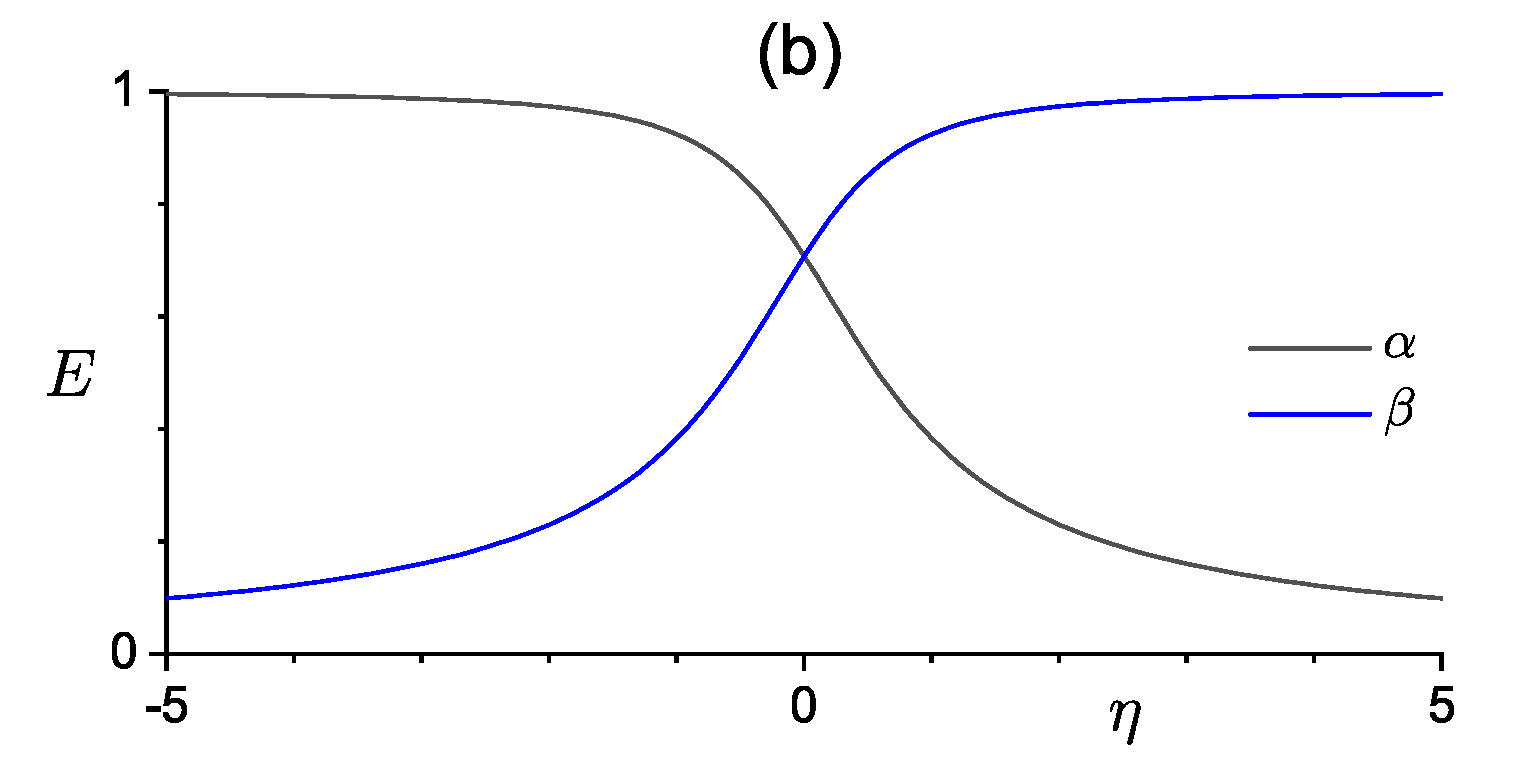
\epsfig{file=TwoLevelABEta.eps,width=\linewidth}
        \end{subfigure}
    	\scaption{
			Dynamika komponent vlastních vektorů pro dvouhladinový systém (a) s proměnnou mimodiagonální interakcí [rovnice~\eqref{eq:TwoLevelXi}], (b) s proměnnou vzdáleností neporušených hladin na diagonále [rovnice~\eqref{eq:TwoLevelEta}].
		}
        \label{fig:TwoLevelAB}
	\end{figure}				

	\begin{figure}[!htbp]
        \begin{subfigure}{0.49\linewidth}
            \centering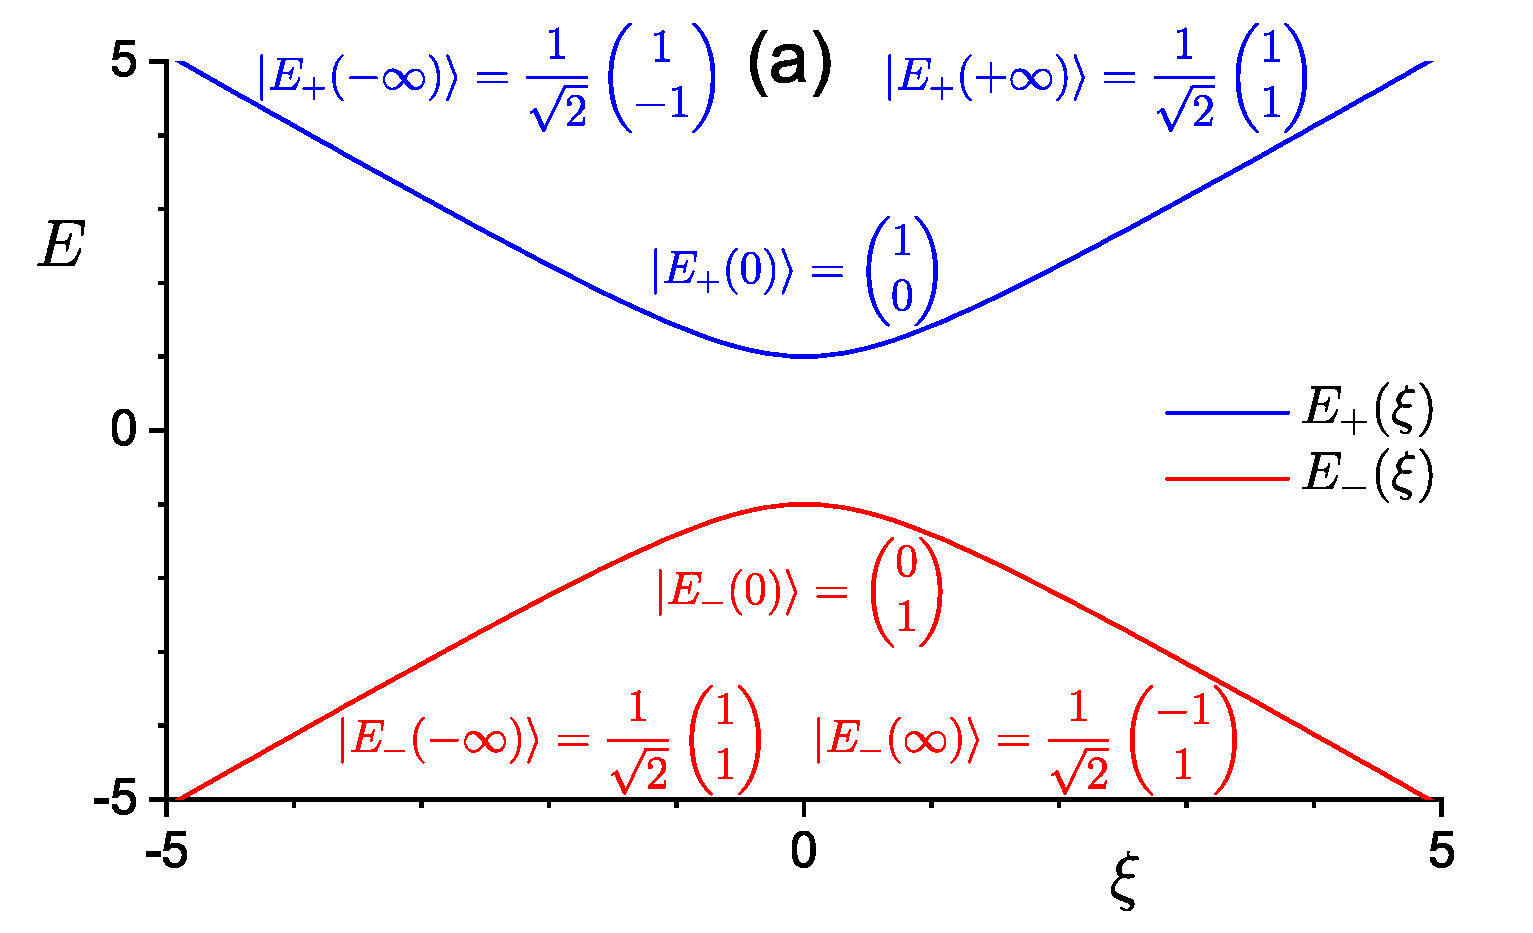
\epsfig{file=TwoLevelXi.eps,width=\linewidth}
        \end{subfigure}
        \hfill
        \begin{subfigure}{0.49\linewidth}
            \centering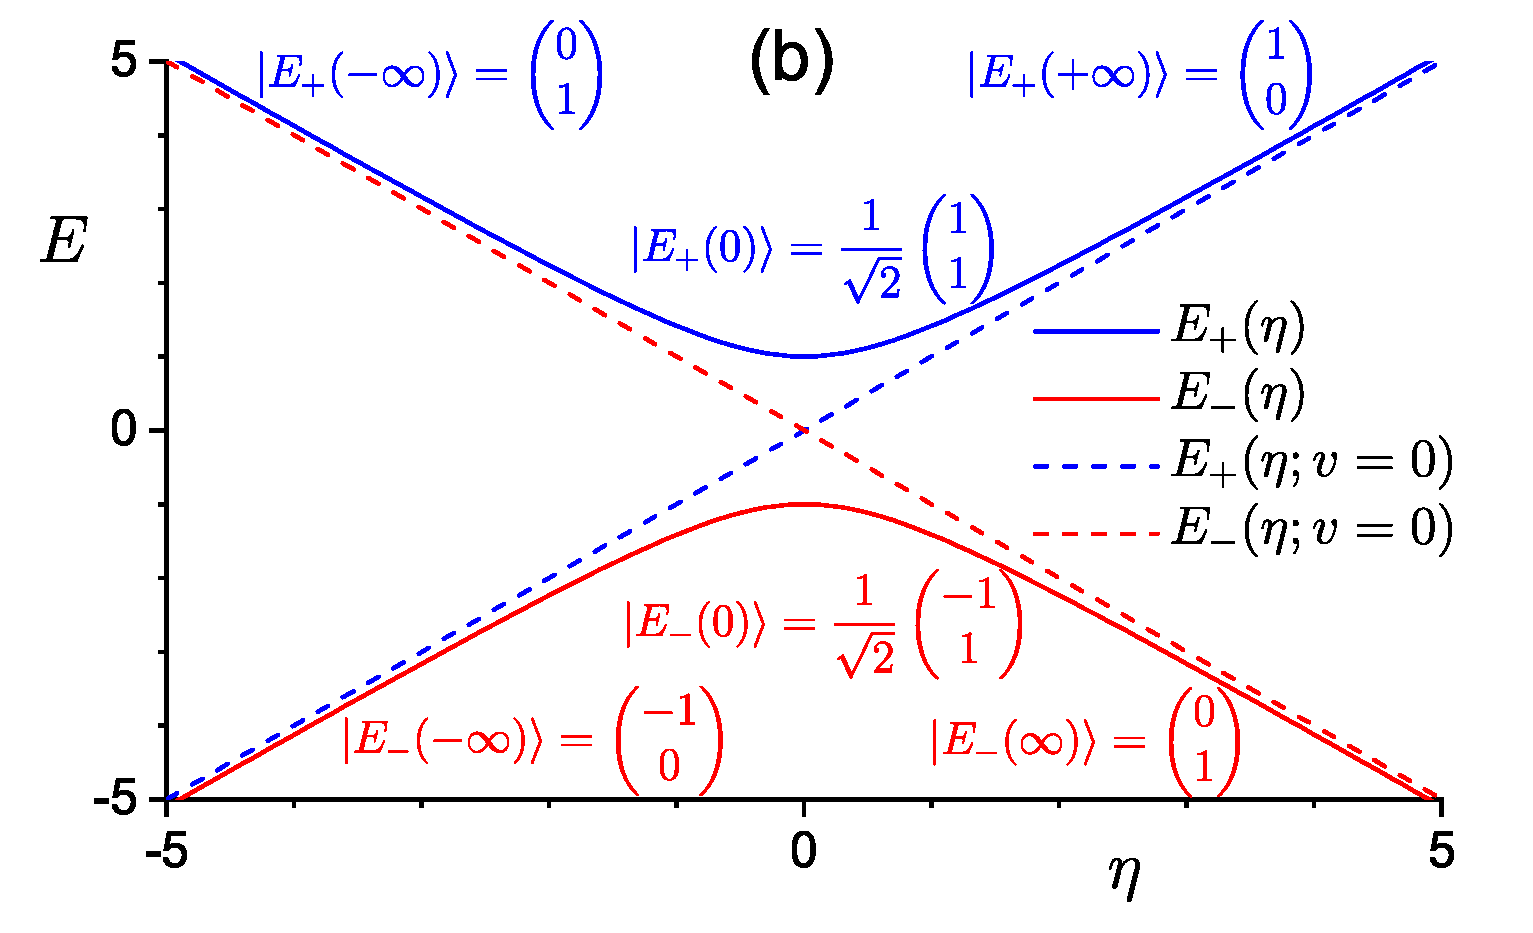
\epsfig{file=TwoLevelEta.eps,width=\linewidth}
        \end{subfigure}
		\scaption{
			Dynamika hladin pro dvouhladinový systém (a) s proměnnou mimodiagonální interakcí, (b) s proměnnou vzdáleností neporušených hladin na diagonále.
		}
    \label{fig:TwoLevelLD}
	\end{figure}				
\end{solution}
